%%%%%%%%%%%%%%%%%%%%%%%%%%%%%%%%%%%%%%%%%%%%%%%%%%%%%%%%%%%%%%%%%%%%%%
% Lớp 11 | Hàm số lượng giác và phương trình lượng giác | Góc lượng giác
% Dạng 1D1?1-5: Đường tròn lượng giác và ứng dụng
% Số câu: 27  (sinh tự động bởi tach_cau.py; từ nay thầy sửa trực tiếp file này)
%%%%%%%%%%%%%%%%%%%%%%%%%%%%%%%%%%%%%%%%%%%%%%%%%%%%%%%%%%%%%%%%%%%%%%

%%%%%%%%%%%%%%%% TRẮC NGHIỆM 4 PHƯƠNG ÁN %%%%%%%%%%%%%%%%

% nguồn: Ok_Toan11_TracNghiem_Lan2
\begin{ex}%[1D1N1-5]%[ma:42bdc646]
	\immini[thm]{Công thức số đo  tổng quát của góc lượng giác $(OA, OM)$ theo độ trong hình bên là
	\choice 
		{$60^{\circ}+k 2\pi$,  $k \in \mathbb{Z}$}
		{$60^{\circ}+k 180^{\circ}$, $k \in  \mathbb{Z}$}
		 {\True $60^{\circ}+k 360^{\circ}$, $k \in \mathbb{Z}$}
		{$-60^{\circ}+k  360^{\circ}$, $k \in \mathbb{Z}$}}
		{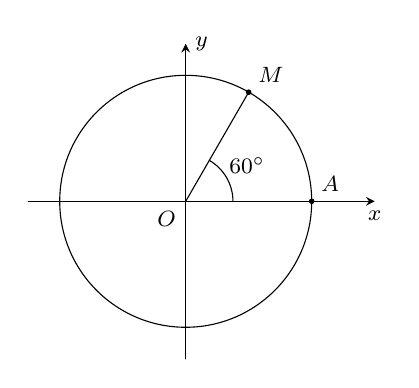
\begin{tikzpicture}[scale=0.8,font=\footnotesize,line join=round,line cap=round,>=stealth]
		 \def\r{2.5}
		\draw[->] (-2.5,0)--(3,0)  node[below]{$x$};
		\draw[->] (0,-2.5)--(0,2.5) node[right]{$y$}; 
		\draw[fill=black] (0,0) node[below left]{$O$} 
			(60:2) circle (1pt)  node[above right]{$M$}
			 (2,0) circle (1pt) node[above right]{$A$};
		\draw  (0:0.3*\r) arc (0:60:0.3*\r);
		\draw  (0,0) circle (2);
		\draw (0,0)--(60:2) 
			 (30:0.45*\r) node{$60^\circ$};
	\end{tikzpicture}
		 }
	 \loigiai{
		Ta có  $(OA,OM)=60^\circ+k 360^{\circ}$, $k \in \mathbb{Z}$.
	} 
\end{ex}

% nguồn: Ok_Toan11_TracNghiem_Lan2
\begin{ex}%[1D1N1-5]%[ma:a6acb348]
	\immini[thm]{Điểm $M$ như hình bên là điểm  biểu diễn cho góc lượng giác nào? Biết $\widehat{AOM}=\dfrac{\pi}{3}$.
	 \choice
		 {$-\dfrac{5\pi}{3}$}
		 {$\dfrac{5\pi}{3}$}
		 {$\dfrac{8\pi}{3}$}
		{\True  $\dfrac{7\pi}{3}$}}
		{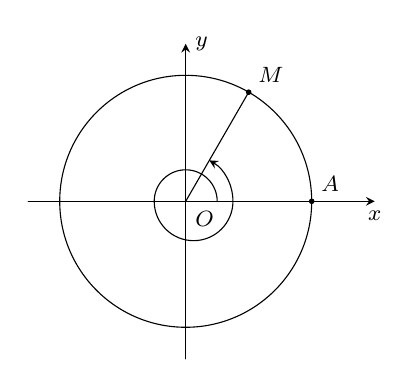
\begin{tikzpicture}[scale=0.8,font=\footnotesize,line join=round,line cap=round,>=stealth]
		 \def\r{2.5}
		\draw[->] (-2.5,0)--(3,0) node[below]{$x$}; 
		 \draw[->] (0,-2.5)--(0,2.5) node[right]{$y$};
		\draw[fill=black] (0,0) node[below  right]{$O$}
			(60:2) circle  (1pt) node[above right]{$M$}
			 (2,0) circle (1pt) node[above right]{$A$};
		\draw (0:0.2*\r)  arc (0:180:0.2*\r)
			(180:0.2*\r) arc (-180:0:0.25*\r); 
		\draw[->]  (0:0.3*\r) arc (0:60:0.3*\r);
		\draw  (0,0) circle (2);
		\draw (0,0)--(60:2); 
	\end{tikzpicture}
		} 
	\loigiai{ 
		Ta có $(OA,OM)=\dfrac{\pi}{3}+2\pi=\dfrac{7\pi}{3}$.  \\
		Suy ra điểm biểu diễn của góc  có số đo $\dfrac{7\pi}{3}$ là điểm $M$ trên đường tròn lượng giác thuộc góc phần tư thứ nhất sao cho $\widehat{AOM}=\dfrac{\pi}{3}$.
	 }
\end{ex}

% nguồn: Ok_Toan11_TracNghiem_Lan2
\begin{ex}%[1D1N1-5]%[ma:3a2e7776]
	\immini[thm]{Điểm $M$ như hình bên  là điểm biểu diễn cho góc lượng giác nào? Biết $\widehat{AOM}=30^\circ$.
	\choice 
		 {\True $390^{\circ}$}
		 {$270^{\circ}$}
		 {$740^{\circ}$}
		 {$-390^{\circ}$}}
		{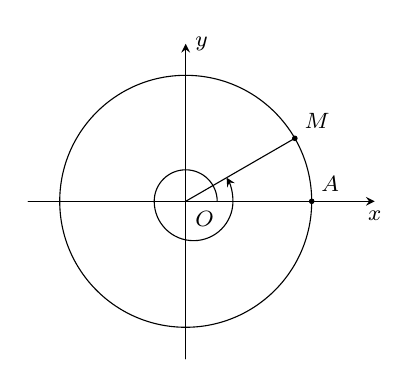
\begin{tikzpicture}[scale=0.8,font=\footnotesize,line join=round,line cap=round,>=stealth]
		\def\r{2.5} 
		\draw[->] (-2.5,0)--(3,0)  node[below]{$x$};
		 \draw[->] (0,-2.5)--(0,2.5) node[right]{$y$};
		\draw[fill=black]  (0,0) node[below right]{$O$}
			(30:2) circle (1pt) node[above  right]{$M$}
			(2,0) circle (1pt) node[above  right]{$A$};
		\draw (0:0.2*\r) arc  (0:180:0.2*\r)
			(180:0.2*\r)  arc (-180:0:0.25*\r);
		\draw[->] (0:0.3*\r) arc (0:30:0.3*\r); 
		\draw (0,0) circle (2); 
		 \draw (0,0)--(30:2);
	\end{tikzpicture}
		 }
	\loigiai{ 
		 Ta có $(OA,OM)=30^{\circ}+360^{\circ}=390^{\circ}$. \\
		Suy ra điểm biểu diễn của góc có  số đo $390^{\circ}$ là điểm $M$ trên đường tròn lượng giác thuộc góc phần tư thứ nhất sao cho $\widehat{AOM}=30^{\circ}$.
	} 
\end{ex}

% nguồn: Ok_Toan11_TracNghiem_Lan2
\begin{ex}%[1D1N1-5]%[ma:4236d208]
	\immini[thm]{Trên đường tròn lượng giác, điểm biểu diễn  của cung $-\dfrac{\pi}{4}$ là
	\choice 
		{$M$} 
		 {$N$}
		 {$P$}
		{\True  $Q$}}
		{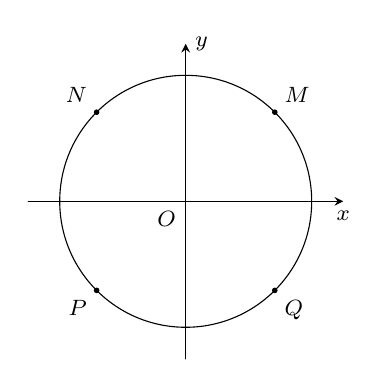
\begin{tikzpicture}[scale=0.8,font=\footnotesize,line join=round,line cap=round,>=stealth]
		\draw[->]  (-2.5,0)--(2.5,0) node[below]{$x$};
		\draw[->] (0,-2.5)--(0,2.5) node[right]{$y$}; 
		\draw[fill=black] (0,0) node[below left]{$O$} 
			(45:2) circle (1pt) node[above right]{$M$} 
			(135:2) circle  (1pt) node[above left]{$N$}
			(-135:2)  circle (1pt) node[below left]{$P$}
			(-45:2) circle  (1pt) node[below right]{$Q$};
		\draw (0,0) circle  (2);
	\end{tikzpicture}
		 }
	\loigiai{ 
		Dựa vào hình vẽ thì điểm biểu  diễn của cung $-\dfrac{\pi}{4}$ là điểm $Q$.
	} 
\end{ex}

% nguồn: Ok_Toan11_TracNghiem_Lan2
\begin{ex}%[1D1H1-5]%[ma:517b86d6]
	Trên đường tròn lượng  giác gốc $A$ cho các góc lượng giác có số đo như sau:
	\begin{enumEX}[I.]{4}
		 \item $\dfrac{\pi}{4}$.
		\item $-\dfrac{7\pi}{4}$. 
		 \item $\dfrac{13\pi}{4}$.
		\item $-\dfrac{71\pi}{4}$. 
	\end{enumEX}
	Hỏi các góc lượng  giác nào có điểm cuối trùng nhau?
	 \choice
		 {Chỉ I và II}
		{Chỉ I, II  và III}
		{Chỉ II,  III và IV}
		{\True  Chỉ I, II và IV}
	\loigiai{ 
		Ta có $\dfrac{\pi}{4}-\left(-\dfrac{7\pi}{4}\right)=2\pi$ nên cung I và II trùng nhau.\\ 
		Vì $\dfrac{\pi}{4}-\left(-\dfrac{71\pi}{4}\right)=18\pi=9\cdot 2\pi$ nên cung I và IV trùng  nhau.
	 }
\end{ex}

% nguồn: Ok_Toan11_TracNghiem_Lan2
\begin{ex}%[1D1H1-5]%[ma:59654732]
	Trên đường tròn lượng giác  gốc $A$ cho các cung có số đo:
	\begin{enumEX}[I.]{4}
		 \item $\dfrac{\pi}{3}$.
		\item $-\dfrac{5\pi}{3}$. 
		 \item $\dfrac{13\pi}{3}$.
		 \item $\dfrac{22\pi}{3}$.
	\end{enumEX}
	Hỏi các cung nào  có điểm cuối trùng nhau?
	 \choice
		{Chỉ I  và II}
		{Chỉ II, III và  IV}
		{\True Chỉ I,  II và III}
		{Chỉ I, II  và IV}
	 \loigiai{
		Ta có  $-\dfrac{5\pi}{3}=\dfrac{\pi}{3}-2\pi$ nên cung $-\dfrac{5\pi}{3}$ và cung $\dfrac{\pi}{3}$ có điểm cuối trùng nhau.\\
	Và $\dfrac{13\pi}{3}=\dfrac{\pi}{3}+4\pi$ nên  cung $\dfrac{13\pi}{3}$ và cung $\dfrac{\pi}{3}$ có điểm cuối trùng nhau.}
\end{ex}

% nguồn: Ok_Toan11_TracNghiem_Lan2
\begin{ex}%[1D1H1-5]%[ma:da71c6b1]
	Trên đường tròn lượng giác, cho góc lượng giác có số đo $\pi$ rad thì mọi góc lượng giác có cùng tia đầu và tia cuối với góc lượng giác trên đều có số đo dạng nào trong các dạng  sau?
	\choice 
		{$-\pi+k \pi$, $(k  \in \mathbb{Z})$}
		{$\pi+k \dfrac{\pi}{2}$, $(k \in \mathbb{Z})$} 
		 {\True $-\pi+k 2\pi$, $(k \in \mathbb{Z})$}
		{$\pi+k \pi$,  $(k \in \mathbb{Z})$}
	\loigiai{ 
		Góc lượng giác có số đo $\pi$ rad thì mọi  góc lượng giác có cùng tia đầu và tia cuối với góc lượng giác trên đều có số đo dạng $\pi+k 2\pi$, $(k \in \mathbb{Z})$ hoặc $-\pi+k 2\pi$, $(k \in \mathbb{Z})$.
	 }
\end{ex}

% nguồn: Ok_Toan11_TracNghiem_Lan2
\begin{ex}%[1D1H1-5]%[ma:94b842de]
	Biểu diễn các góc lượng giác $\alpha=-\dfrac{5\pi}{6}$, $\beta=\dfrac{\pi}{3}$, $\gamma=\dfrac{25\pi}{3}$, $\delta=\dfrac{19\pi}{6}$ trên đường tròn lượng giác. Các góc nào có  điểm biểu diễn trùng nhau?
	 \choice
		{\True $\beta$ và $\gamma$; $\alpha$  và $\delta$}
		 {$\alpha$, $\beta$, $\gamma$}
		{$\beta$,  $\gamma$, $\delta$}
		{$\alpha$  và $\beta$; $\gamma$ và $\delta$}
	 \loigiai{
		\begin{itemize}
			\item \textbf{Cách  1.} \\
			Ta có $\delta-\alpha=4\pi$, suy ra $2$ cung $\alpha$ và $\delta$  có điểm cuối trùng nhau.\\
			 Và $\gamma-\beta=8\pi$, suy ra hai cung $\beta$ và $\gamma$ có điểm cuối trùng nhau.
			\item  \textbf{Cách 2.} \\
			Gọi là điểm cuối của các cung  $\alpha$, $\beta$, $\gamma$, $\delta$.\\
			Biểu diễn các cung trên đường  tròn lượng giác ta có $B\equiv C$, $A\equiv D$.
		\end{itemize}
	} 
\end{ex}

% nguồn: Ok_Toan11_TracNghiem_Lan2
\begin{ex}%[1D1H1-5]%[ma:0bf7bf59]
	Trên đường tròn lượng giác, cho góc lượng giác có số đo $\dfrac{3\pi}{2}$ rad thì mọi góc lượng giác có cùng tia  đầu và tia cuối với góc lượng giác trên đều có số đo dạng nào trong các dạng sau?
	\choice 
		{$\dfrac{3\pi}{2}+k \pi$,  $(k \in \mathbb{Z})$}
		{$-\dfrac{3\pi}{2}+k \pi$, $(k \in  \mathbb{Z})$}
		{\True $-\dfrac{\pi}{2}+k  2\pi$, $(k \in \mathbb{Z})$}
		 {$-\dfrac{3\pi}{2}+k 2\pi$, $(k \in \mathbb{Z})$}
	\loigiai{ 
		Góc lượng giác có số đo $\dfrac{3\pi}{2}$ rad thì mọi góc lượng giác có cùng  tia đầu và tia cuối với góc lượng giác trên đều có số đo dạng $\dfrac{3\pi}{2}+k 2\pi$, $(k \in \mathbb{Z})$ hoặc $-\dfrac{\pi}{2}+k 2\pi$, $(k \in \mathbb{Z})$.
	} 
\end{ex}

% nguồn: Ok_TracNghiemLop11_Lan1
\begin{ex}%[1D1H1-5]%[ma:b46f0d9f]
	Góc nào trong các góc sau có điểm biểu diễn là  $M\left(-\dfrac{\sqrt{3}}{2};-\dfrac{1}{2} \right)$?
	 \choice
		{$-\dfrac{\pi}{3}+k2\pi  \left(k\in \mathbb{Z}\right)$}
		{\True $\dfrac{7\pi}{6}+k2\pi \left(k\in \mathbb{Z}\right)$} 
		{$\dfrac{2\pi}{3}+k2\pi  \left(k\in \mathbb{Z}\right)$}
		{$-\dfrac{\pi}{6}+k2\pi  \left(k\in \mathbb{Z}\right)$}
	\loigiai{ 
		Ta có $M\left(-\dfrac{\sqrt{3}}{2};-\dfrac{1}{2} \right)$ nên $M$ thuộc góc phần  tư thứ ba.\\
		Gọi $H$ là hình  chiếu của $M$ trên $Ox$.\\
		 Khi đó $\cos \widehat{MOH}=\dfrac{OH}{OM}=\dfrac{\dfrac{\sqrt{3}}{2}}{1}=\dfrac{\sqrt{3}}{2} \Rightarrow \widehat{MOH}=\dfrac{\pi}{6}$.\\
		Vậy góc có điểm biểu diễn là $M\left(-\dfrac{\sqrt{3}}{2};-\dfrac{1}{2} \right)$ có số đo $\dfrac{\pi}{6}+\pi+k2\pi=\dfrac{7\pi}{6}+k2\pi  \, \left(k\in \mathbb{Z}\right)$.
	} 
\end{ex}

% nguồn: Ok_TracNghiemLop11_Lan1
\begin{ex}%[1D1V1-5]%[ma:5b8a7ef0]
	Biết một góc lượng giác $\left(Ou,Ov\right)$ có số đo là $\dfrac{2021\pi}{3}$, số đo của góc hình học  $uOv$ là
	 \choice
		{$\dfrac{2\pi}{3}$} 
		{\True $\dfrac{\pi}{3}$} 
		{$\dfrac{\pi}{6}$} 
		 {$\dfrac{-\pi}{3}$}
	 \loigiai{
		\begin{itemize}
			\item Khi $Ou,Ov$ đối nhau thì một góc lượng giác $\left(Ou,Ov\right)$ có  số đo là $\pi$ rad và góc hình học $uOv$ cũng có số đo là $\pi$ rad.
			\item Khi $Ou,Ov$ không đối nhau thì số đo góc hình học $uOv$ là $\beta$ rad $\left(0\le \beta < \pi \right)$ và góc  lượng giác $\left(Ou,Ov\right)$ có số đo là $\beta+k2\pi$ hoặc $-\beta+k2\pi$ với $k\in \mathbb{Z}$, tức là
			sđ$\left(Ou,Ov\right)=\alpha+k2\pi$, với $\left|\alpha \right|=\beta$  và $k\in \mathbb{Z}$.
			\item Ta có sđ$\left(Ou,Ov\right)=\dfrac{2021\pi}{3}=\dfrac{-\pi}{3}+674\pi=\dfrac{-\pi}{3}+337\cdot  2\pi$.
		\end{itemize}
		Vậy góc lượng giác $\left(Ou,Ov\right)$ có số đo bằng $\dfrac{2021\pi}{3}$, thì số đo góc hình học  $uOv$ là $\dfrac{\pi}{3}$.
	} 
\end{ex}


%%%%%%%%%%%%%%%% ĐÚNG/SAI %%%%%%%%%%%%%%%%

% nguồn: Ok_dungsai_lop11_Lan1
\begin{ex}%[1D1N1-5]%[ma:a3b9dbc7]
  \immini{
 Cho đường tròn lượng giác có điểm gốc là điểm $A$ (tham  khảo hình bên). Mỗi khẳng định sau đúng hay sai?
 \choiceTF 
  {\True Điểm biểu diễn góc lượng giác  có số đo $\dfrac{\pi}{4}$ nằm trên cung $AB$}
  {Điểm biểu diễn góc lượng giác có số đo  $\dfrac{-\pi}{3}$ nằm trên cung $BA'$}
   {Điểm biểu diễn góc lượng giác có số đo $\dfrac{4\pi}{5}$ nằm trên cung $A'B'$}
   {Điểm biểu diễn góc lượng giác có số đo $-\dfrac{5\pi}{9}$ nằm trên cung $B'A$}}
  {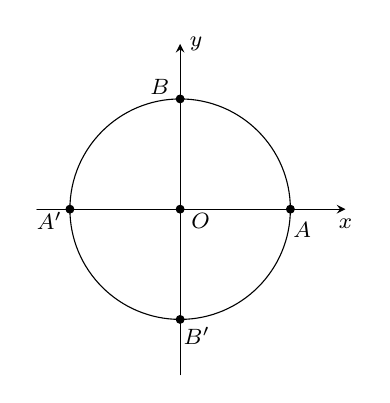
\begin{tikzpicture}[scale=1.4,font=\footnotesize,line join=round,line cap=round,>=stealth]
  \draw[->] (-1.3,0)--(1.5,0) node[below]{$x$}; 
   \draw[->] (0,-1.5)--(0,1.5) node[right]{$y$};
   \path
   (1,0) coordinate (A) 
    (0:0) coordinate (O)
    (-1,0) coordinate (A')
   (0,1) coordinate  (B)
   (0,-1)  coordinate (B');
  \draw 
   (O) circle  (1);
  \foreach \p/\g  in {A/-60,O/-30,A'/-150,B/150,B'/-45}
  \draw[fill=black]  (\p) circle (1pt) node[shift=(\g:3mm)] {$\p$};
 \end{tikzpicture}
  } 
 \loigiai{ 
  \begin{itemchoice}
   \itemch Điểm biểu diễn góc lượng giác có số đo $\dfrac{\pi}{4}$ nằm trên cung $AB$. 
   \itemch Điểm biểu diễn góc lượng giác có số đo $\dfrac{-\pi}{3}$ nằm trên cung $B'A$. 
   \itemch  Điểm biểu diễn góc lượng giác có số đo $\dfrac{4\pi}{5}$ nằm trên cung $BA'$.
   \itemch Điểm biểu diễn góc lượng giác có số đo $-\dfrac{5\pi}{9}$  nằm trên cung $A'B'$.
  \end{itemchoice}
 } 
\end{ex}

% nguồn: Ok_dungsai_lop11_Lan1
\begin{ex}%[1D1H1-5]%[ma:700ec352]
 \immini{ Trên đường tròn lượng giác với điểm gốc là $A$. Điểm $M$ thuộc đường tròn sao cho cung $AM$ có số đo $60^\circ$ (tham khảo hình vẽ bên). Gọi $N,P,Q$ lần lượt là các điểm đối xứng  với điểm $M$ qua gốc tọa độ, trục $Oy$ và trục $Ox$, $A'$ là điểm đối xứng với $A$ qua gốc tọa độ $O$. Mỗi khẳng định dưới đây đúng hay sai?
  \choiceTF
  {\True Số đo của cung lượng giác $AP$ bằng $120^\circ+ k360^\circ$, $k\in\mathbb{Z}$} 
  {\True Số đo của cung lượng giác $AQ$  bằng $-30^\circ+ k360^\circ$, $k\in\mathbb{Z}$}
  {\True Số đo của  cung lượng giác $AA'$ bằng $180^\circ+ k360^\circ$, $k\in\mathbb{Z}$}
  { Số đo của cung lượng giác $AN$ bằng $120^\circ+ k360^\circ$, $k\in\mathbb{Z}$} 
  } 
  {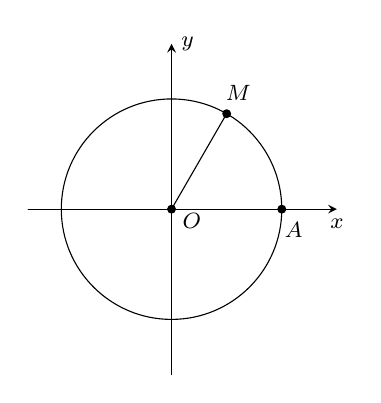
\begin{tikzpicture}[scale=1.4,font=\footnotesize,line join=round,line cap=round,>=stealth]
  \draw[->] (-1.3,0)--(1.5,0) node[below]{$x$}; 
  \draw[->]  (0,-1.5)--(0,1.5) node[right]{$y$};
  \path 
   (1,0) coordinate  (A)
   (0:0) coordinate (O) 
   (60:1)  coordinate (M)
   (120:1) coordinate  (P)
   (240:1) coordinate (N) 
   (-60:1) coordinate  (Q)
    (-1,0) coordinate (A');
  \draw 
    (O) circle (1)
   (O)--(M); 
  \foreach  \p/\g in {A/-60,O/-30,M/60}
  \draw[fill=black] (\p) circle (1pt) node[shift=(\g:3mm)]  {$\p$};
 \end{tikzpicture}
   }
 \loigiai{ 
 \immini{ 
  \begin{itemchoice}
   \itemch Ta có $\widehat{AOP}=120^\circ$ nên số đo của cung lượng  giác $AP$ bằng \break $120^\circ+ k360^\circ$, $k\in\mathbb{Z}$.
   \itemch Ta có $\widehat{AOQ}=30^\circ$  nên số đo của cung lượng giác $AQ$ bằng \break $-30^\circ+ k360^\circ$, $k\in\mathbb{Z}$.
   \itemch Ta  có $\widehat{AOA'}=180^\circ$ nên số đo của cung lượng giác $AA'$ bằng \break $180^\circ+ k360^\circ$, $k\in\mathbb{Z}$.
   \itemch Ta có $\widehat{AON}=120^\circ$ nên số đo của cung lượng giác $AA'$ bằng \break  $-120^\circ+ k360^\circ$, $k\in\mathbb{Z}$.
  \end{itemchoice}
  }{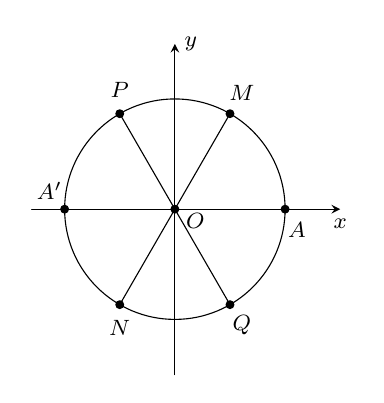
\begin{tikzpicture}[scale=1.4,font=\footnotesize,line join=round,line cap=round,>=stealth]
   \draw[->] (-1.3,0)--(1.5,0) node[below]{$x$};
   \draw[->] (0,-1.5)--(0,1.5) node[right]{$y$};
   \path
   (1,0)  coordinate (A)
    (0:0) coordinate (O)
   (60:1) coordinate (M) 
    (120:1) coordinate (P)
   (240:1)  coordinate (N)
    (-60:1) coordinate (Q)
   (-1,0)  coordinate (A');
   \draw
    (O) circle (1)
   (O)--(M) 
   (O)--(P) 
    (O)--(N)
   (O)--(Q); 
  \foreach  \p/\g in {A/-60,O/-30,M/60,P/90,N/-90,Q/-60,A'/130}
  \draw[fill=black] (\p) circle (1pt) node[shift=(\g:3mm)]  {$\p$};
 \end{tikzpicture}
  } 
 } 
\end{ex}

% nguồn: Ok_dungsai_lop11_Lan1
\begin{ex}%[1D1H1-5]%[ma:41ad4c6e]
 Các góc có cùng điểm biểu diễn  trên đường tròn lượng giác \textbf{ĐÚNG} hay \textbf{SAI}?
 \choiceTF 
  {\True $756 ^{\circ}$, $-324 ^{\circ}$} 
  {\True $-324 ^{\circ}$, $ 36 ^{\circ}$} 
  {$36 ^{\circ}$,$  216 ^{\circ}$}
   {\True $-\dfrac{41\pi}{7}$, $\dfrac{15\pi}{7}$}
  \loigiai{
  Ta có 
  $$ \begin{aligned}
  756  ^{\circ}&=36 ^{\circ}+2\cdot 360 ^{\circ}\\
   -324 ^{\circ}&=36 ^{\circ}-360 ^{\circ}\\
  216  ^{\circ}&=-144 ^{\circ}+ 360 ^{\circ}\\
   -\dfrac{41\pi}{7}&=-\dfrac{42\pi-\pi}{7}=\dfrac{\pi}{7}-6\pi\\
   \dfrac{15\pi}{7}&=\dfrac{\pi+14\pi}{7}=\dfrac{\pi}{7}+2\pi
 \end{aligned}$$
  Nên
 \begin{itemchoice}
  \itemch $756 ^{\circ}$ và  $-324 ^{\circ}$ có cùng điểm biểu diễn trên trường tròn lượng giác.
  \itemch $36^{\circ}$ và $-324 ^{\circ}$ có cùng điểm biểu diễn trên trường  tròn lượng giác.
  \itemch $36^{\circ}$  và $216^{\circ}$ không có cùng điểm biểu diễn trên trường tròn lượng giác.
  \itemch $ -\dfrac{41\pi}{7}$ và $\dfrac{15\pi}{7}$ có cùng điểm biểu diễn trên trường  tròn lượng giác.
 \end{itemchoice}
} 
\end{ex}

% nguồn: Ok_dungsai_lop11_Lan1
\begin{ex}%[1D1H1-5]%[ma:8bfca71f]
 \immini{Biểu diễn góc lượng giác trên đường tròn lượng  giác. Các mệnh đề sau \textbf{ĐÚNG} hay \textbf{SAI} ?
 \choiceTF 
  {$36 ^{\circ}+k360 ^{\circ}, \, k\in \mathbb{Z}$ là điểm $M$  thuộc góc phần tư thứ $II$}
  {\True $-60 ^{\circ}+k180  ^{\circ},\, k\in \mathbb{Z}$ là các điểm $M_1$, $M_2$ thuộc góc phần tư thứ $II$ và $IV$}
  {$-\dfrac{\pi}{4}+k2\pi$, $ k\in \mathbb{Z}$  là $M$ thuộc góc phần tư thứ $III$}
   {\True $-\dfrac{\pi}{6}+k\dfrac{\pi}{2}$, $ k\in \mathbb{Z}$ là bốn điểm $M$, $N$, $P$, $Q$ thuộc góc phần tư thứ $I$, $II$, $III$, $IV$}}{
  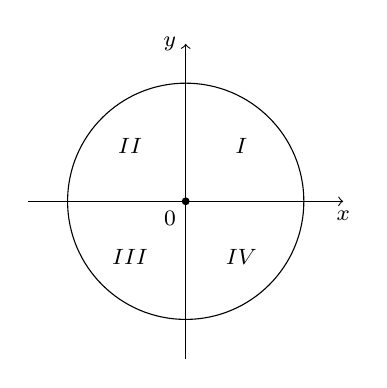
\begin{tikzpicture}[font=\footnotesize]
    \draw[->] (180:2)--(0:2)  node[below] {$x$};
    \draw[->] (-90:2)--(90:2) node[left] {$y$}; 
     \draw (0:0) circle (1.5);
    \fill (0:0) circle  (0.05) node[below left] {$0$};
    \node at  (45:1) {$I$};
    \node  at (135:1) {$II$};
    \node at (225:1) {$III$}; 
     \node at (-45:1) {$IV$};
   \end{tikzpicture}
   }
  \loigiai{
  \begin{itemchoice}
   \itemch \immini{Xét góc lượng giác $k360  ^{\circ}$, dù $k$ là số chẵn hay số lẻ thì góc này cũng có điểm biểu diễn là điểm $A$ (điểm gốc trên đường tròn lượng giác).
   Vì vậy, góc lượng giác $36 ^{\circ}+k360 ^{\circ}$ có điểm biểu diễn là điểm $M$ thuộc  góc phần tư thứ $I$ của đường tròn lượng giác và $\widehat{AOM}=36 ^{\circ}$.}
    {
   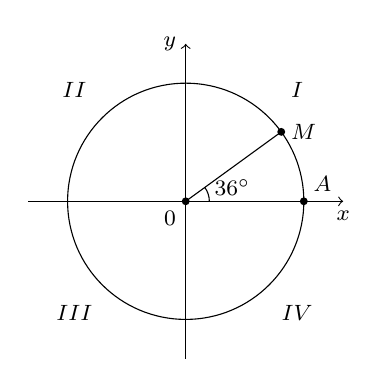
\begin{tikzpicture}[font=\footnotesize]
     \draw[->]  (180:2)--(0:2) node[below] {$x$};
     \draw[->] (-90:2)--(90:2) node[left]  {$y$};
     \draw (0:0) circle (1.5); 
     \fill (0:0) circle (0.05) node[below  left] {$0$};
     \node at (45:2)  {$I$};
     \node  at (135:2) {$II$};
     \node  at (225:2) {$III$};
      \node at (-45:2) {$IV$};
     \fill (36:1.5) circle (0.05)  node[right] {$M$};
     \fill (0:1.5)  circle (0.05) node[above right] {$A$};
      \draw (0:0)--(36:1.5)
      (0:0.3) arc (0:36:0.3)  node[right] {$36^\circ$};
    \end{tikzpicture}
   } 
   \itemch \immini{Xét góc lượng giác $k180 ^{\circ}$. Nếu $k$ chẵn thì  góc này có điểm biểu diễn là $A(1;0)$, nếu $k$ lẻ thì góc này có điểm biểu diễn là điểm $B(-1;0)$.
   Vì vậy, $-60 ^{\circ}+k180 ^{\circ}$ có các điểm biểu diễn là $M_1$ và $M_2$ như hình vẽ  bên.}
   { 
   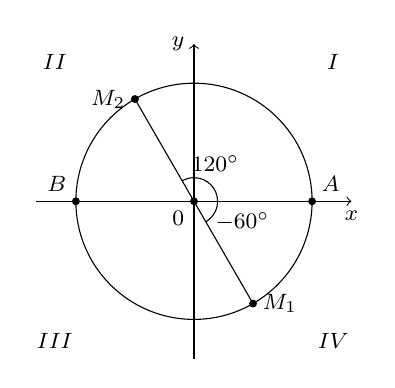
\begin{tikzpicture}[font=\footnotesize]
     \draw[->] (180:2)--(0:2)  node[below] {$x$};
     \draw[->] (-90:2)--(90:2)  node[left] {$y$};
     \draw  (0:0) circle (1.5);
     \fill (0:0) circle  (0.05) node[below left] {$0$};
     \node at (45:2.5)  {$I$};
     \node at  (135:2.5) {$II$};
     \node at (225:2.5) {$III$}; 
     \node at (-45:2.5) {$IV$}; 
     \fill  (-60:1.5) circle (0.05) node[right] {$M_1$};
     \fill (120:1.5) circle (0.05) node[left]  {$M_2$};
     \fill (0:1.5) circle (0.05) node[above  right] {$A$};
      \fill (180:1.5) circle (0.05) node[above left] {$B$};
     \draw  (0:0)--(-60:1.5)
      (0:0.3) arc (0:-60:0.3)  node[right] {$-60^\circ$};
     \draw (0:0)--(120:1.5) 
      (0:0.3) arc (0:120:0.3) node[above right] {$120^\circ$}; 
    \end{tikzpicture}
    }
   \itemch \immini{ Ta biết góc lượng giác $k2\pi$ luôn có điểm biểu diễn là $A(1;0)$, vì vậy góc lượng  giác $-\dfrac{\pi}{4}+k2\pi$ có điểm biểu diễn là $M$ thuộc góc phần tư thứ IV và thoả mãn $\widehat{AOM}=\dfrac{\pi}{4}$.}
   { 
   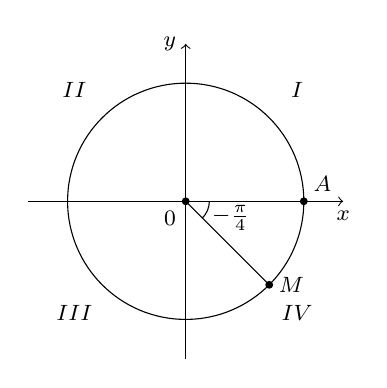
\begin{tikzpicture}[font=\footnotesize]
      \draw[->] (180:2)--(0:2) node[below] {$x$};
      \draw[->] (-90:2)--(90:2) node[left] {$y$};
     \draw  (0:0) circle (1.5);
     \fill (0:0) circle (0.05) node[below left]  {$0$};
     \node at (45:2)  {$I$};
      \node at (135:2) {$II$};
     \node at (225:2)  {$III$};
      \node at (-45:2) {$IV$};
     \fill (-45:1.5) circle (0.05) node[right] {$M$}; 
     \fill  (0:1.5) circle (0.05) node[above right] {$A$};
      \draw (0:0)--(-45:1.5)
      (0:0.3)  arc (0:-45:0.3) node[right] {$-\frac{\pi}{4}$};
    \end{tikzpicture}
   } 
   \itemch \immini{Xét góc lượng giác $k\dfrac{\pi}{2}$. Khi $k=0$ thì $k\dfrac{\pi}{2}=0$, góc này có điểm  biểu diễn là điểm $A(1;0)$. Khi $k=1$ thì $k\dfrac{\pi}{2}=\dfrac{\pi}{2}$, góc này có điểm biểu diễn là điểm $C(0;1)$.
   Khi $k=2$ thì $k\dfrac{\pi}{2}=\pi$, góc này có điểm biểu  diễn là điểm $B(-1;0)$.
   Khi $k=3$ thì $k\dfrac{\pi}{2}=\dfrac{3\pi}{2}$, góc  này có điểm biểu diễn là điểm $D(0;-1)$. Nếu $k=4,5,6,\ldots$ thì ta thấy rằng các điểm biểu diễn có được vẫn là sự lặp lại của $A,B,C,D$.
   Vì vậy điểm biểu diễn của $-\dfrac{\pi}{6}+k\dfrac{\pi}{2}$ là bốn điểm $M,N,P,Q$ trên  đường tròn lượng giác (xem hình vẽ trên).} {
   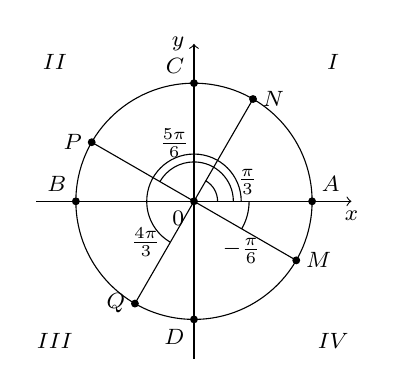
\begin{tikzpicture}[font=\footnotesize]
     \draw[->] (180:2)--(0:2) node[below] {$x$}; 
     \draw[->] (-90:2)--(90:2) node[left] {$y$}; 
     \draw  (0:0) circle (1.5);
     \fill (0:0) circle (0.05) node[below left] {$0$}; 
     \node at  (45:2.5) {$I$};
      \node at (135:2.5) {$II$};
     \node  at (225:2.5) {$III$};
     \node  at (-45:2.5) {$IV$};
     \fill (60:1.5) circle (0.05) node[right] {$N$}; 
     \fill (-30:1.5) circle (0.05) node[right] {$M$}; 
     \fill (150:1.5) circle (0.05) node[left]  {$P$};
     \fill (240:1.5) circle  (0.05) node[left] {$Q$};
     \fill  (0:1.5) circle (0.05) node[above right] {$A$};
     \fill (180:1.5) circle (0.05) node[above  left] {$B$};
     \fill (90:1.5) circle (0.05) node[above left] {$C$}; 
     \fill  (-90:1.5) circle (0.05) node[below left] {$D$};
      \draw (0:0)--(60:1.5)
      (0:0.3) arc (0:60:0.3); 
     \node[right] at (30:0.5) {$\frac{\pi}{3}$}; 
     \draw (0:0)--(150:1.5) 
      (0:0.5) arc (0:150:0.5);  \node[above] at (120:0.5) {$\frac{5\pi}{6}$};
     \draw (0:0)--(240:1.5) 
      (0:0.6) arc  (0:240:0.6) node[left] {$\frac{4\pi}{3}$};
     \draw  (0:0)--(-30:1.5)
      (0:0.7)  arc (0:-30:0.7) node[below] {$-\frac{\pi}{6}$};
    \end{tikzpicture}
    }
  \end{itemchoice}
 } 
\end{ex}

% nguồn: Ok_dungsai_lop11_Lan1
\begin{ex}%[1D1H1-5]%[ma:b5c177c8]
 Các cặp góc sau có cùng điểm biểu diễn  trên đường tròn lượng giác \textbf{ĐÚNG} hay \textbf{SAI} ?
  \choiceTF
  {\True  $1127 ^{\circ}{,}-313 ^{\circ}$}
   {$1127 ^{\circ}{,}-674$}
  {\True  $\dfrac{61\pi}{5}{,}-\dfrac{19\pi}{5}$}
   {$\dfrac{61\pi}{5}{,}-\dfrac{23\pi}{4}$}
  \loigiai{
  \begin{itemchoice}
   \itemch Ta có $1127 ^{\circ}=47 ^{\circ}+3\cdot360 ^{\circ}$; $ -313 ^{\circ}=47 ^{\circ}-360  ^{\circ}$.\\
   Vì vậy các góc lượng giác $1127 ^{\circ}{,}-313 ^{\circ}$ có cùng một điểm biểu diễn và điểm này trùng với điểm biểu diễn của góc  $47 ^{\circ}$ trên đường tròn lượng giác.
   \itemch Ta có $-674 ^{\circ}=46 ^{\circ}-2\cdot 360 ^{\circ}$  nên không trùng điểm biểu diễn với góc $1127^\circ$.
   \itemch Ta có:  $\dfrac{61\pi}{5}=\dfrac{\pi}{5}+6\cdot2\pi$; $-\dfrac{19\pi}{5}=\dfrac{\pi}{5}-2\cdot 2\pi$.\\
   Vì vậy các góc lượng giác $\dfrac{61\pi}{5}$ , $-\dfrac{19\pi}{5}$ có cùng một điểm biểu diễn và điểm này trùng với điểm biểu diễn của góc $\dfrac{\pi}{5}$ trên đường tròn lượng  giác.
   \itemch Ta  có $-\dfrac{23\pi}{4}=\dfrac{\pi}{4}-3\cdot 2\pi$ nên không trùng điểm biểu diễn với góc $\dfrac{61\pi}{5}$.
  \end{itemchoice}
  }
\end{ex}

% nguồn: Ok_dungsai_lop11_Lan2
\begin{ex}%[1D1H1-5]%[ma:a877d381]
	Các góc có cùng điểm  biểu diễn trên đường tròn lượng giác là
	\choiceTF 
		{\True  $1\,127^\circ$, $-313^\circ$}
		{$1\,127^\circ$, $-674^\circ$} 
		{\True  $\dfrac{61\pi}{5}$, $-\dfrac{19 \pi}{5}$}
		{$\dfrac{61\pi}{5}$, $-\dfrac{23\pi}{4}$} 
	\loigiai{ 
		\begin{itemchoice}
			 \itemch \textbf{Đúng.}\\
			 Ta có $1\,127^\circ=47^\circ+3\cdot360^\circ$;\\
			$-313^\circ=47^\circ-360^\circ$.\\ 
			Vì vậy các góc lượng giác $1\,127^\circ$, $-313^\circ$ có cùng một điểm biểu diễn và điểm  này trùng với điểm biểu diễn của góc $47^\circ$ trên đường tròn lượng giác.
			\itemch \textbf{Sai.}\\ 
			Ta có $1\,127^\circ=47^\circ+3\cdot360^\circ$;\\ 
			$-674^\circ=46^\circ-2\cdot360^\circ$. 
			Vì vậy các góc lượng giác $1\,127^\circ$, $-674^\circ$ không cùng  một điểm biểu diễn trên đường tròn lượng giác.
			 \itemch \textbf{Đúng.}\\
			 Ta có $\dfrac{61 \pi}{5}=\dfrac{\pi}{5}+6\cdot2 \pi$;\\
			$-\dfrac{19  \pi}{5}=\dfrac{\pi}{5}-2\cdot2 \pi$.\\
			Vì vậy các góc lượng giác $\dfrac{61 \pi}{5}$, $-\dfrac{19 \pi}{5}$ có cùng một điểm biểu diễn và điểm này trùng với  điểm biểu diễn của góc $\dfrac{\pi}{5}$ trên đường tròn lượng giác.
			\itemch  \textbf{Sai.}\\
			Ta có $\dfrac{61 \pi}{5}=\dfrac{\pi}{5}+6\cdot2 \pi$;\\ 
			$-\dfrac{23  \pi}{4}=\dfrac{\pi}{4}-3\cdot2 \pi$.\\
			Vì vậy các góc lượng  giác $\dfrac{61 \pi}{5}$, $-\dfrac{23\pi}4$ không cùng một điểm biểu diễn trên đường tròn lượng giác.
		\end{itemchoice}
	} 
\end{ex}

% nguồn: Ok_dungsai_lop11_Lan2
\begin{ex}%[1D1H1-5]%[ma:c46d9c75]
	Biểu diễn góc lượng giác trên đường  tròn lượng giác. Khi đó
	\choiceTF 
		{$36^\circ+k360^\circ$, $k\in  \mathbb{Z}$ là điểm $M$ thuộc góc phần tư thứ II}
		{\True $-60^\circ+k180^\circ$, $k\in \mathbb{Z}$ là các điểm $M_1$,  $M_2$ thuộc góc phần tư thứ II và IV}
		{$-\dfrac{\pi}{4}+k2\pi$, $k\in \mathbb{Z}$ là $M$ thuộc góc phần tư thứ  III}
		{\True $-\dfrac{\pi}{6}+k\dfrac{\pi}{2}$, $k\in \mathbb{Z}$ là bốn điểm $M$,  $N$, $P$, $Q$ thuộc góc phần tư thứ I, II, III, IV}
	\loigiai{ 
		\begin{itemchoice}
			\itemch \textbf{Sai.} 
		\immini{ 
			Xét góc lượng giác $k 360^\circ$, dù $k$ là số  chẵn hay số lẻ thì góc này cũng có điểm biểu diễn là điểm $A$ (điểm gốc trên đường tròn lượng giác).\\
			Vì vậy, góc lượng giác $36^\circ+k 360^\circ$ có điểm biểu diễn là điểm $M$ thuộc góc phần tư thứ I  của đường tròn lượng giác và $\widehat{AOM}=36^\circ$.
			}{ 
			\begin{tikzpicture}[scale=.8,>=stealth,font=\footnotesize,line join=round,line cap=round]
					\draw[fill=black](0,0) coordinate (O)  node[below left]{$O$} circle (1pt)
						(2,0) coordinate (A) node[above right]  {$A$} circle (1pt)
						(36:2) coordinate (M) node  [right] {$M$} circle (1pt);
					\draw[very  thick] (0,0) circle (2 cm);
					\draw[->] (-3,0)--(3,0)  node [below]{$x$};
					 \draw[->] (0,-3)--(0,3) node [left]{$y$};
					\clip  (-3.5,-3.5) rectangle (3.5,3.5);
					\draw (3,3) node {I} 
						(-3,3) node  {II}
						(-3,-3) node  {III}
						(3,-3)  node {IV};
					\draw  (M)--(O);
					\pic [draw,->,angle eccentricity=3] {angle =  A--O--M};
				\end{tikzpicture}
			 }
			\itemch \textbf{Đúng.} 
		 \immini{
			Xét góc lượng giác $k180^\circ$. Nếu $k$ chẵn thì góc này có điểm biểu diễn là  $A(1; 0)$, nếu $k$ lẻ thì góc này có điểm biểu diễn là điểm $B(-1; 0)$.\\
			Vì vậy, $-60^\circ+k 180^\circ$ có các điểm biểu diễn  là ${M_1}$ và ${M_2}$ như hình vẽ.
			 }{
			\begin{tikzpicture}[scale=.8,>=stealth,font=\footnotesize,line join=round,line cap=round]
					\draw[fill=black](0,0) coordinate  (O) node[below left]{$O$} circle (1pt)
						(2,0) coordinate (A)  node[above right] {$A$} circle (1pt)
						(-60:2) coordinate (M) node [below  right] {$M_1$} circle (1pt)
						(120:2) coordinate (N) node  [above left] {$M_2$} circle (1pt);
					 \draw[very thick] (0,0) circle (2 cm);
					 \draw[->] (-3,0)--(3,0) node [below]{$x$};
					\draw[->] (0,-3)--(0,3)  node [left]{$y$};
					\clip (-3.5,-3.5) rectangle (3.5,3.5); 
					\draw (3,3)  node {I}
						(-3,3) node  {II}
						(-3,-3) node {III} 
						(3,-3) node  {IV};
					\draw  (M)--(O)--(N);
					\pic  [draw,->,angle eccentricity=3] {angle = A--O--N};
					\pic [draw,<-,angle eccentricity=3] {angle = M--O--A}; 
				\end{tikzpicture}
			} 
			\itemch  \textbf{Sai.}
		 \immini{
			Ta biết góc lượng giác $k2\pi$ luôn có điểm biểu diễn là $A(1;0)$,  vì vậy góc lượng giác $-\dfrac{\pi}4+k 2\pi$ có điểm biểu diễn là $M$ thuộc góc phần tư thứ IV và thoả mãn $\widehat{AOM}=\dfrac{\pi}4$.
			}{ 
			\begin{tikzpicture}[scale=.8,>=stealth,font=\footnotesize,line join=round,line cap=round]
					\draw[fill=black](0,0) coordinate (O) node[below left]{$O$}  circle (1pt)
						(2,0) coordinate (A) node[above right] {$A$} circle (1pt) 
						(-45:2) coordinate (M) node  [right] {$M$} circle (1pt);
					\draw[very thick] (0,0)  circle (2 cm);
					\draw[->]  (-3,0)--(3,0) node [below]{$x$};
					\draw[->] (0,-3)--(0,3) node  [left]{$y$};
					\clip (-3.5,-3.5) rectangle  (3.5,3.5);
					\draw  (3,3) node {I}
						(-3,3) node  {II}
						(-3,-3) node  {III}
						 (3,-3) node {IV};
					 \draw (M)--(O);
					 \pic [draw,<-,angle eccentricity=3]{angle = M--O--A};
				\end{tikzpicture}
			 }
			 \itemch \textbf{Đúng.}
		\immini{ 
			Xét góc lượng giác $k \dfrac{\pi}{2}$. Khi $k=0$ thì $k \dfrac{\pi}{2}=0$, góc này có điểm biểu diễn là điểm $A(1; 0)$. Khi $k=1$ thì $k \dfrac{\pi}{2}=\dfrac{\pi}{2}$, góc này có điểm biểu diễn là điểm $C(0; 1)$. Khi $k=2$ thì $k \dfrac{\pi}{2}=\pi$, góc này có điểm biểu diễn là điểm $B(-1; 0)$. Khi $k=3$ thì $k \dfrac{\pi}{2}=\dfrac{3 \pi}{2}$, góc này có điểm biểu diễn là điểm $D(0;-1)$. Nếu $k=4,5,6, \ldots$ thì ta thấy rằng các điểm biểu diễn có được  vẫn là sự lặp lại của $A$, $B$, $C$, $D$.\\
			Vì vậy điểm biểu diễn của $-\dfrac{\pi}{6}+k \dfrac{\pi}{2}$ là bốn  điểm $M$, $N$, $P$, $Q$ trên đường tròn lượng giác.
			}{ 
			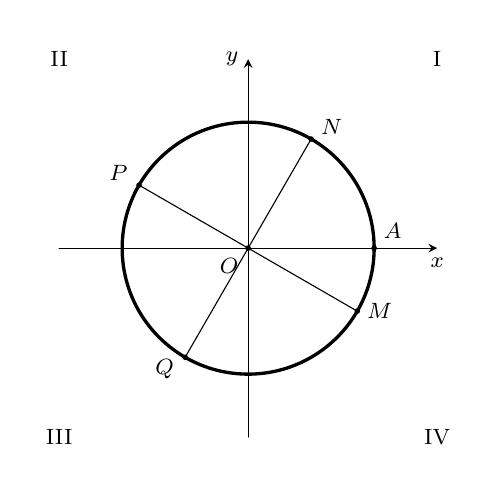
\begin{tikzpicture}[scale=.8,>=stealth,font=\footnotesize,line join=round,line cap=round]
					\draw[fill=black](0,0) coordinate (O) node[below left]{$O$} circle (1pt) 
						(2,0) coordinate (A) node[above right]  {$A$} circle (1pt)
						(-30:2) coordinate (M) node [right] {$M$}  circle (1pt);
					 \draw[very thick] (0,0) circle (2 cm);
					 \draw[->] (-3,0)--(3,0) node [below]{$x$};
					\draw[->] (0,-3)--(0,3) node [left]{$y$}; 
					\coordinate (N) at  (60:2);
					\coordinate (P) at  (150:2);
					 \coordinate (Q) at (240:2);
					\clip (-3.5,-3.5)  rectangle (3.5,3.5);
					\draw (3,3) node {I} 
						(-3,3) node {II} 
						 (-3,-3) node {III}
						(3,-3)  node {IV};
					\draw  (M)--(P)
						(N)--(Q); 
					\foreach \p/\g in {N/30,P/150,Q/-150}\draw[fill=black] (\p) circle (1pt) node[shift={(\g:.3)},scale=1]{$\p$}; 
				\end{tikzpicture}
			} 
		\end{itemchoice}
	} 
\end{ex}

% nguồn: Ok_dungsai_lop11_Lan2
\begin{ex}%[1D1H1-5]%[ma:42842829]
	Biểu diễn góc lượng giác trên đường tròn lượng  giác. Khi đó
	 \choiceTF
		{\True  $125^\circ$ là điểm $M$ thuộc góc phần tư thứ thứ II}
		{$405^\circ$ là điểm $N$ thuộc góc phần tư thứ  III}
		{$\dfrac{19 \pi}{3}$ là  điểm $P$ thuộc góc phần tư thứ II}
		{\True $-\dfrac{13 \pi}{6}$  là điểm $Q$ thuộc góc phần tư thứ IV}
	 \loigiai{
		\begin{itemchoice}
			 \itemch \textbf{Đúng.}\\
		\immini{ 
			Điểm biểu diễn của  góc lượng giác có số đo ${125^\circ}$ là điểm ${M}$ thuộc góc phần tư thứ thứ II của đường tròn lượng giác thoả mãn $\widehat{AOM}={{125}^\circ}$.
			 }{
			\begin{tikzpicture}[scale=.8,>=stealth,font=\footnotesize,line join=round,line cap=round]
					\draw[fill=black](0,0) coordinate (O) node[below  left]{$O$} circle (1pt)
						(2,0) coordinate (A) node[above right] {$A$}  circle (1pt)
						(125:2) coordinate (M) node [left] {$M$} circle  (1pt);
					\draw[very thick] (0,0)  circle (2 cm);
					\draw[->]  (-3,0)--(3,0) node [below]{$x$};
					\draw[->]  (0,-3)--(0,3) node [left]{$y$};
					 \clip (-3.5,-3.5) rectangle (3.5,3.5);
					\draw  (3,3) node {I}
						(-3,3)  node {II}
						(-3,-3) node  {III}
						(3,-3) node {IV}; 
					\draw  (M)--(O);
					\pic [draw,->,angle eccentricity=3]  {angle = A--O--M};
				\end{tikzpicture}
			 }
			\itemch \textbf{Sai.} 
		 \immini{
			Ta có $405^\circ=45^\circ+360^\circ$. Vì  vậy điểm biểu diễn của góc lượng giác $405^\circ$ là điểm $N$ thuộc góc phần tư thứ I của đường tròn lượng giác và thoả mãn $\widehat{AON}=45^\circ$.
			}{ 
			\begin{tikzpicture}[scale=.8,>=stealth,font=\footnotesize,line join=round,line cap=round]
					\draw[fill=black](0,0) coordinate (O) node[below  left]{$O$} circle (1pt)
						(2,0) coordinate (A) node[above  right] {$A$} circle (1pt)
						(45:2) coordinate (M)  node [right] {$N$} circle (1pt);
					\draw[very thick] (0,0)  circle (2 cm);
					\draw[->]  (-3,0)--(3,0) node [below]{$x$};
					\draw[->] (0,-3)--(0,3) node [left]{$y$}; 
					\clip (-3.5,-3.5)  rectangle (3.5,3.5);
					 \draw (3,3) node {I}
						(-3,3) node {II} 
						(-3,-3) node  {III}
						 (3,-3) node {IV};
					\draw  (M)--(O);
					\pic [draw,->,angle eccentricity=3]  {angle = A--O--M};
				\end{tikzpicture}
			} 
			 \itemch \textbf{Sai.}
		\immini{ 
			Ta  có $\dfrac{19\pi}{3}=\dfrac{18\pi+\pi}{3}=\dfrac{\pi}{3}+3\cdot2 \pi$. Vì vậy điểm biểu diễn của góc lượng giác $\dfrac{19 \pi}{3}$ là điểm $P$ thuộc góc phần tư thứ I của đường tròn lượng giác và thoả mãn $\widehat{AOP}=\dfrac{\pi}{3}$.
			}{ 
			\begin{tikzpicture}[scale=.8,>=stealth,font=\footnotesize,line join=round,line cap=round]
					\draw[fill=black](0,0) coordinate (O) node[below left]{$O$} circle  (1pt)
						(2,0) coordinate (A) node[above right]  {$A$} circle (1pt)
						(60:2) coordinate (M)  node [right] {$P$} circle (1pt);
					 \draw[very thick] (0,0) circle (2 cm);
					\draw[->] (-3,0)--(3,0)  node [below]{$x$};
					\draw[->]  (0,-3)--(0,3) node [left]{$y$};
					\clip  (-3.5,-3.5) rectangle (3.5,3.5);
					 \draw (3,3) node {I}
						(-3,3)  node {II}
						(-3,-3)  node {III}
						(3,-3)  node {IV};
					\draw  (M)--(O);
					\pic [draw,->,angle eccentricity=3] {angle  = A--O--M};
				\end{tikzpicture}
			} 
			 \itemch \textbf{Đúng.}
		 \immini{
			Ta có $-\dfrac{13 \pi}{6}=\dfrac{-12 \pi-\pi}{6}=-\dfrac{\pi}{6}-2 \pi$. Vì vậy điểm biểu diễn của góc lượng giác $-\dfrac{13 \pi}{6}$ là điểm  $Q$ thuộc góc phần tư thứ IV của đường tròn lượng giác và thoả mãn $\widehat{AOQ}=\dfrac{\pi}{6}$.
			 }{
			\begin{tikzpicture}[scale=.8,>=stealth,font=\footnotesize,line join=round,line cap=round]
					\draw[fill=black](0,0) coordinate (O)  node[below left]{$O$} circle (1pt)
						(2,0)  coordinate (A) node[above right] {$A$} circle (1pt)
						(30:2) coordinate (M) node [right] {$Q$} circle  (1pt);
					\draw[very thick]  (0,0) circle (2 cm);
					\draw[->] (-3,0)--(3,0) node  [below]{$x$};
					\draw[->] (0,-3)--(0,3)  node [left]{$y$};
					\clip (-3.5,-3.5)  rectangle (3.5,3.5);
					 \draw (3,3) node {I}
						(-3,3) node  {II}
						(-3,-3)  node {III}
						(3,-3)  node {IV};
					\draw (M)--(O); 
					\pic  [draw,->,angle eccentricity=3] {angle = A--O--M};
				\end{tikzpicture}
			 }
		\end{itemchoice}
	} 
\end{ex}

% nguồn: Ok_dungsai_lop11_Lan2
\begin{ex}%[1D1H1-5]%[ma:8b0bca24]
	Các góc có  cùng điểm biểu diễn trên đường tròn lượng giác là
	\choiceTF 
		{\True $756^\circ$, $-324^\circ$} 
		 {\True $-324^\circ$, $36^\circ$}
		 {$36^\circ$, $216^\circ$}
		 {\True $-\dfrac{41 \pi}{7}$, $\dfrac{15 \pi}{7}$}
	\loigiai{ 
		\begin{itemchoice}
			 \itemch \textbf{Đúng.}\\
			Ta có $756^\circ=36^\circ+2 \cdot 360^\circ$; $-324^\circ=36^\circ-360^\circ$. Vậy ba góc lượng giác gồm $756^\circ$, $-324^\circ$ có cùng một điểm biểu diễn trên đường  tròn lượng giác.
			\itemch  \textbf{Đúng.}\\
			Ta có $-324^\circ=36^\circ-360^\circ$. Vậy  ba góc lượng giác gồm $-324^\circ$, $36^\circ$ có cùng một điểm biểu diễn trên đường tròn lượng giác.
			\itemch  \textbf{Sai.}\\
			 Hiển nhiên.
			\itemch  \textbf{Đúng.}\\
			Ta có $-\dfrac{41 \pi}{7}=-\dfrac{42 \pi-\pi}{7}=\dfrac{\pi}{7}-6  \pi$; $\dfrac{15 \pi}{7}=\dfrac{\pi+14 \pi}{7}=\dfrac{\pi}{7}+2 \pi$.
			 Vậy hai góc lượng giác là $-\dfrac{41 \pi}{7}$, $\dfrac{15 \pi}{7}$ có cùng một điểm biểu diễn, điểm đó trùng với điểm biểu diễn của góc $\dfrac{\pi}{7}$ trên đường tròn lượng giác.
		\end{itemchoice}
	} 
\end{ex}

% nguồn: Ok_dungsai_lop11_Lan2
\begin{ex}%[1D1H1-5]%[ma:336160d4]
	 Biểu diễn các góc lượng giác có số đo sau đây trên đường tròn lượng giác. Khi đó
	 \choiceTF
		{\True Điểm biểu diễn của góc  lượng giác có số đo $218^\circ$ là điểm $M$ thuộc góc phần tư thứ III của đường tròn lượng giác thoả mãn $\widehat{AOM}=218^\circ$}
		{Điểm biểu diễn của góc lượng giác có số đo $-405^\circ$  là điểm $N$ thuộc góc phần tư thứ IV của đường tròn lượng giác thoả mãn $\widehat{AON}=-45^\circ$}
		{\True Điểm biểu diễn của góc lượng giác có số đo $\dfrac{25 \pi}{4}$ là điểm $P$ thuộc  góc phần tư thứ I của đường tròn lượng giác thoả mãn $\widehat{AOP}=\dfrac{\pi}{4}$}
		{Điểm biểu diễn của góc lượng giác có số đo $\dfrac{15 \pi}{2}$ là điểm $Q(0;-1)$ thuộc đường tròn lượng giác thoả  mãn $\widehat{AOQ}=-\dfrac{\pi}{2}$}
	\loigiai{ 
		\begin{itemchoice}
			\itemch \textbf{Đúng.} 
		\immini{ 
			Điểm biểu diễn của góc lượng giác có số  đo $218^\circ$ là điểm ${M}$ thuộc góc phần tư thứ III của đường tròn lượng giác thoả mãn $\widehat{A O M}=218^\circ$.
			}{ 
			\begin{tikzpicture}[scale=.8,>=stealth,font=\footnotesize,line join=round,line cap=round]
					 \draw[fill=black](0,0) coordinate (O)
						(2,0) coordinate (A) node[above right] {$A$}  circle (1pt);
					\coordinate (M)  at (218:2);
					 \draw[very thick] (0,0) circle (2 cm);
					 \draw[->] (-3,0)--(3,0) node [below]{$x$};
					\draw[->] (0,-3)--(0,3) node  [left]{$y$};
					\clip (-3.5,-3.5)  rectangle (3.5,3.5);
					 \draw (3,3) node {I}
						(-3,3) node {II} 
						(-3,-3) node {III} 
						(3,-3)  node {IV};
					 \draw (M)--(O);
					\pic [draw,->,angle eccentricity=3] {angle = A--O--M}; 
					\foreach \p/\g in {O/45,M/-150}\draw[fill=black] (\p) circle (1pt)  node[shift={(\g:.3)},scale=1]{$\p$};
				\end{tikzpicture}
			} 
			\itemch \textbf{Sai.} 
		\immini{ 
			Ta có $-405^\circ=-45^\circ-360^\circ$. Điểm biểu diễn của góc lượng giác có số đo $-405^\circ$ là điểm $N$ thuộc góc phần tư thứ IV của  đường tròn lượng giác thoả mãn $\widehat{AON}=45^\circ$.
			}{ 
			\begin{tikzpicture}[scale=.8,>=stealth,font=\footnotesize,line join=round,line cap=round]
					 \draw[fill=black](0,0) coordinate (O)
						(2,0) coordinate (A) node[above right] {$A$} circle (1pt); 
					\coordinate (N) at (45:2); 
					\draw[very  thick] (0,0) circle (2 cm);
					\draw[->] (-3,0)--(3,0) node  [below]{$x$};
					 \draw[->] (0,-3)--(0,3) node [left]{$y$};
					\clip  (-3.5,-3.5) rectangle (3.5,3.5);
					\draw  (3,3) node {I}
						(-3,3)  node {II}
						(-3,-3)  node {III}
						 (3,-3) node {IV};
					 \draw (N)--(O);
					\pic [draw,->,angle eccentricity=3] {angle = A--O--N}; 
					\foreach \p/\g in {O/-45,N/30}\draw[fill=black]  (\p) circle (1pt) node[shift={(\g:.3)},scale=1]{$\p$};
				\end{tikzpicture}
			} 
			\itemch  \textbf{Đúng.}
		 \immini{
			Ta có $\dfrac{25 \pi}{4}=\dfrac{\pi+24 \pi}{4}=\dfrac{\pi}{4}+6 \pi$. Điểm biểu diễn của góc lượng giác có số đo $\dfrac{25 \pi}{4}$ là điểm $P$ thuộc góc phần tư thứ I của đường  tròn lượng giác thoả mãn $\widehat{AOP}=\dfrac{\pi}{4}$.
			 }{
			\begin{tikzpicture}[scale=.8,>=stealth,font=\footnotesize,line join=round,line cap=round]
					\draw[fill=black](0,0) coordinate  (O)
						(2,0) coordinate (A) node[above right] {$A$} circle  (1pt);
					\coordinate  (P) at (45:2);
					\draw[very thick] (0,0) circle (2  cm);
					\draw[->] (-3,0)--(3,0) node  [below]{$x$};
					\draw[->] (0,-3)--(0,3) node  [left]{$y$};
					\clip  (-3.5,-3.5) rectangle (3.5,3.5);
					\draw  (3,3) node {I}
						(-3,3)  node {II}
						(-3,-3) node {III} 
						(3,-3)  node {IV};
					\draw (P)--(O); 
					\pic [draw,->,angle eccentricity=3] {angle =  A--O--P};
					\foreach \p/\g in {O/-45,P/45}\draw[fill=black] (\p) circle (1pt)  node[shift={(\g:.3)},scale=1]{$\p$};
				\end{tikzpicture}
			} 
			 \itemch \textbf{Sai.}
		 \immini{
			Ta có $\dfrac{15 \pi}{2}=\dfrac{16 \pi-\pi}{2}=-\dfrac{\pi}{2}+8 \pi$. Điểm biểu diễn của góc lượng giác có số đo ${\dfrac{15 \pi}{2}}$ là điểm $Q(0;-1)$ thuộc đường  tròn lượng giác thoả mãn $\widehat{AOQ}=\dfrac{\pi}{2}$.
			}{ 
			\begin{tikzpicture}[scale=.8,>=stealth,font=\footnotesize,line join=round,line cap=round]
					\draw[fill=black](0,0) coordinate (O) 
						(2,0) coordinate (A) node[above right] {$A$}  circle (1pt);
					\coordinate (Q) at  (90:2);
					\draw[very  thick] (0,0) circle (2 cm);
					\draw[->] (-3,0)--(3,0) node [below]{$x$}; 
					 \draw[->] (0,-3)--(0,3) node [left]{$y$};
					\clip (-3.5,-3.5)  rectangle (3.5,3.5);
					 \draw (3,3) node {I}
						(-3,3) node  {II}
						 (-3,-3) node {III}
						(3,-3) node {IV}; 
					\draw (Q)--(O); 
					\pic [draw,->,angle eccentricity=3]  {angle = A--O--Q};
					\foreach \p/\g in {O/45,Q/45}\draw[fill=black] (\p)  circle (1pt) node[shift={(\g:.3)},scale=1]{$\p$};
				\end{tikzpicture}
			 }
		\end{itemchoice}
	} 
\end{ex}

% nguồn: Ok_dungsai_lop11_Lan1
\begin{ex}%[1D1V1-5]%[ma:3c1c8699]
 Biểu diễn góc lượng giác trên đường tròn lượng giác.  Khi đó
  \choiceTF
  {$36^{^\circ}+k360^{^\circ}, k\in \mathbb{Z}$ là điểm $M$ thuộc góc phần tư  thứ $II$}
  {\True $-60^{^\circ}+k180^{^\circ}, k\in \mathbb{Z}$ là các điểm $M_1, M_2$ thuộc góc phần tư thứ $II$  và $IV$}
  {$-\dfrac{\pi}{4}+k2\pi, k\in \mathbb{Z}$ là $M$ thuộc  góc phần tư thứ $III$}
  {\True $-\dfrac{\pi}{6}+k\dfrac{\pi}{2}, k\in \mathbb{Z}$ là bốn điểm $M,N,P,Q$ thuộc góc phần tư thứ  $I,II,III,IV$}
  \loigiai{
  \begin{itemchoice}
   \itemch 
   \immini{{\bf Sai.}\\
   Xét góc lượng giác $k360^{^\circ}$, dù $k$ là số chẵn hay số lẻ  thì góc này cũng có điểm biểu diễn là điểm $A$ (điểm gốc trên đường tròn lượng giác).\\
   Vì vậy, góc lượng giác $36^{^\circ}+k360^{^\circ}$ có điểm biểu  diễn là điểm $M$ thuộc góc phần tư thứ $I$ của đường tròn lượng giác và $\widehat{AOM}=36^{^\circ}$.}
   {\begin{tikzpicture}[scale=0.6,font=\footnotesize,line join=round,line cap=round,>=stealth]
  \path (0,0) coordinate (O) 
   (3,0) coordinate (A) 
   (0,3)  coordinate (B)
   (0,-3)  coordinate (B')
   (-3,0) coordinate (A') 
    (0:0)++(36:3) coordinate (M);
  \draw[->] (-4,0) -- (4,0) node[above,blue]{$x$}; 
   \draw[->] (0,-4) -- (0.,4) node[left,blue]{$y$};
  \draw[blue]  (O) circle (3cm);
  \draw[rotate=0,->,green!50!black] (0.5,0)  arc (0:36:0.5cm);
  \draw[green!50!black]  (M)--(O);
  \foreach \p/\r in  {A/-45,M/75,O/-150,A'/-135,B'/-45,B/45}
  \fill  (\p) circle (1pt) node[shift={(\r:3mm)},blue]{$\p$};
  \draw  pic[draw=none,"$36^\circ$",angle radius=10mm]{angle=A--O--M};
 \end{tikzpicture}
    }
   \itemch \immini{{\bf  Đúng.}\\
   Xét góc lượng giác $k180^{^\circ}$. Nếu $k$ chẵn thì góc này có điểm biểu diễn là $A(1;0)$, nếu $k$ lẻ  thì góc này có điểm biểu diễn là điểm $B(-1;0)$.\\
   Vì vậy, $-60^{^\circ}+k180^{^\circ}$ có các điểm biểu diễn là $M_1$ và  $M_2$ như hình vẽ bên.}
   {\begin{tikzpicture}[scale=0.6,font=\footnotesize,line join=round,line cap=round,>=stealth]
  \path (0,0) coordinate (O) 
   (3,0)  coordinate (A)
    (0,3) coordinate (B)
   (0,-3)  coordinate (B')
   (-3,0)  coordinate (A')
   (0:0)++(-60:3) coordinate (M_1) 
    ($2*(O)-(M_1)$) coordinate (M_2);
   \draw[->] (-4,0) -- (4,0) node[above,blue]{$x$};
  \draw[->] (0,-4) --  (0.,4) node[left,blue]{$y$};
  \draw[blue] (O)  circle (3cm);
   \draw[rotate=0,->,green!50!black] (0.5,0) arc (0:-60:0.5cm);
  \draw[rotate=0,->,green!50!black,dashed] ((0.5,0) arc  (0:120:0.5cm);
   \draw[green!50!black] (M_1)--(M_2);
  \foreach \p/\r in {A/-45,M_1/-45,O/-150,A'/-135,B'/-45,B/45,M_2/135} 
  \fill (\p) circle (1pt)  node[shift={(\r:3mm)},blue]{$\p$};
   \draw pic[draw=none,"$-60^\circ$",angle radius=10mm]{angle=M_1--O--A}
   pic[draw=none,"$120^\circ$",angle  radius=10mm]{angle=A--O--M_2};
 \end{tikzpicture}
   } 
   \itemch  \immini{{\bf Sai.}\\
   Ta biết góc lượng giác $k2\pi$ luôn có điểm biểu diễn là $A(1;0)$, vì vậy góc lượng  giác $-\dfrac{\pi}{4}+k2\pi$ có điểm biểu diễn là $M$ thuộc góc phần tư thứ IV và thoả mãn $\widehat{AOM}=\dfrac{\pi}{4}$.}
   {\begin{tikzpicture}[scale=0.6,font=\footnotesize,line join=round,line cap=round,>=stealth]
  \path (0,0) coordinate (O) 
   (3,0) coordinate (A) 
   (0,3)  coordinate (B)
   (0,-3) coordinate  (B')
   (-3,0) coordinate  (A')
   (0:0)++(-45:3) coordinate (M); 
  \draw[->] (-4,0) -- (4,0) node[above,blue]{$x$}; 
  \draw[->] (0,-4) --  (0.,4) node[left,blue]{$y$};
  \draw[blue] (O) circle (3cm); 
   \draw[rotate=0,->,green!50!black] (0.5,0) arc (0:-45:0.5cm);
  \draw[green!50!black]  (M)--(O);
  \foreach \p/\r  in {A/-45,M/-45,O/-150,A'/-135,B'/-45,B/45}
  \fill (\p)  circle (1pt) node[shift={(\r:3mm)},blue]{$\p$};
  \draw  pic[draw=none,"$-\frac{\pi}{4}$",angle radius=10mm]{angle=M--O--A};
 \end{tikzpicture}
   } 
    \itemch \immini{{\bf Đúng.}\\
   Xét góc lượng giác $k\dfrac{\pi}{2}$. Khi $k=0$ thì $k\dfrac{\pi}{2}=0$, góc này có  điểm biểu diễn là điểm $A(1;0)$. Khi $k=1$ thì $k\dfrac{\pi}{2}=\dfrac{\pi}{2}$, góc này có điểm biểu diễn là điểm $C(0;1)$. Khi $k=2$ thì $k\dfrac{\pi}{2}=\pi$, góc này có điểm biểu diễn là điểm $B(-1;0)$. Khi $k=3$ thì $k\dfrac{\pi}{2}=\dfrac{3\pi}{2}$, góc này có điểm biểu diễn là điểm $D(0;-1)$. Nếu $k=4,5,6,\ldots$ thì ta thấy rằng các điểm biểu diễn có được vẫn là sự lặp lại của $A,B,C,D$.\\
   Vì vậy điểm biểu diễn của $-\dfrac{\pi}{6}+k\dfrac{\pi}{2}$ là bốn điểm $M,N,P,Q$ trên đường tròn lượng giác (xem hình  vẽ trên).}
   {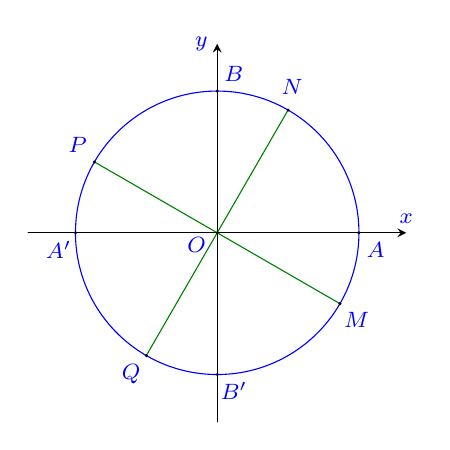
\begin{tikzpicture}[scale=0.6,font=\footnotesize,line join=round,line cap=round,>=stealth]
  \path (0,0)  coordinate (O)
   (3,0)  coordinate (A)
    (0,3) coordinate (B)
   (0,-3)  coordinate (B')
    (-3,0) coordinate (A')
   (0:0)++(-30:3) coordinate (M) 
    (0:0)++(60:3) coordinate (N)
   (0:0)++(150:3)  coordinate (P)
   (0:0)++(240:3)  coordinate (Q);
  \draw[->] (-4,0) -- (4,0) node[above,blue]{$x$}; 
  \draw[->] (0,-4) --  (0.,4) node[left,blue]{$y$};
  \draw[blue]  (O) circle (3cm);
   \draw[green!50!black] (M)--(P)
   (N)--(Q); 
  \foreach  \p/\r in {A/-45,M/-45,O/-150,A'/-135,B'/-45,B/45,N/80,P/135,Q/-130}
  \fill (\p) circle  (1pt) node[shift={(\r:3mm)},blue]{$\p$};
 \end{tikzpicture}
   } 
  \end{itemchoice}
  }
\end{ex}


%%%%%%%%%%%%%%%% TRẢ LỜI NGẮN %%%%%%%%%%%%%%%%

% nguồn: Ok_TraLoiNgan_Lop11_Lan2
\begin{ex}%[1D1H1-5]%[ma:94d416ab]
	 Huyện lị Quản Bạ tỉnh Hà Giang và huyện lị Cái Nước tỉnh Cà Mau cùng nằm ở $105^{\circ}$ kinh đông, nhưng Quản Bạ ở $23^{\circ}$ vĩ bắc, Cái Nước ở vĩ độ $9^{\circ}$ bắc. Hãy tính độ dài cung kinh tuyến nối hai huyện lị đó (khoảng cách theo đường chim bay), coi Trái Đất có bán kính $6378$ km.
	\loigiai{ 
	\shortans{1558} 
		Góc ở tâm chắn cung kinh tuyến nối huyện Quản Bạ tỉnh Hà Giang và huyện Cái Nước tỉnh Cà Mau có số đo bằng  $23^{\circ}-9^{\circ}=14^{\circ}$. \\
		Vậy độ dài cung  kinh tuyến đó bằng $\dfrac{6378\cdot 14\cdot \pi}{180} \approx 1558$ km.
	 }
\end{ex}

% nguồn: Ok_TraLoiNgan_Lop11_Lan2
\begin{ex}%[1D1H1-5]%[ma:5982efae]
	\immini[thm]{Một chiếc đồng hồ có kim giờ và kim phút được cho như trong hình vẽ sau. Xét tia $Ou$ là kim  giờ, $Ov$ là kim phút. Xét chiều quay của góc là chiều kim đồng hồ, khi đó số đo của góc lượng giác $(Ou, Ov)$ là}
	{\begin{tikzpicture}[scale=0.8,font=\footnotesize,line join=round,line cap=round,>=stealth]
		 \def\r{2.5}
		 \path
			(0,0) coordinate  (O)
			(30:2.5)  coordinate (A)
			 (180:2.5) coordinate (B)
			(-30:2.5)  coordinate (C)
			 (60:2) coordinate (M)
			(-135:2) coordinate  (N);
		\draw[line width=1.5pt] (O)--(180:1) 
			 (O) circle (2pt);
		 \draw[line width=1pt] (O)--(90:2);
		\draw[line width=2pt] (0,0)  circle (3);
		\foreach \x/\g in {1/60,2/30,3/0,4/-30,5/-60,6/-90,7/-120,8/-150,9/-180,10/-210,11/-240,12/90} 
		\fill (\g:2.4) circle (1pt) 
			($(\g:2.7)$) node {$\x$}; 
	\end{tikzpicture}
	 }
	\shortans{90} 
	 \loigiai{
		Ta có $(Ou,  Ov)=90^{\circ}$.
	} 
\end{ex}

% nguồn: Ok_TraLoiNgan_Lop11_Lan2
\begin{ex}%[1D1H1-5]%[ma:8e367613]
	Kim giờ  dài $6$ cm và kim phút dài $11$ cm của đồng hồ chỉ $4$ giờ. Hỏi thời gian ít nhất để $2$ kim vuông góc với nhau là bao nhiêu? (Kết quả làm tròn đến hàng phần trăm).
	 \shortans{0,09}
	 \loigiai{
		Một giờ, kim phút quét được một góc lượng giác $2\pi$;  kim giờ quét được một góc $\dfrac{\pi}{6}$. Hiệu vận tốc giữa kim phút và kim giờ là $2\pi-\dfrac{\pi}{6}=\dfrac{11\pi}{6}$.\\
		Vào lúc 4 giờ hai kim tạo với  nhau một góc là $\dfrac{2\pi}{3}$.\\
		 Khoảng thời gian ít nhất để hai kim vuông góc với nhau là $\left(\dfrac{2\pi}{3}-\dfrac{\pi}{2}\right): \dfrac{11\pi}{6}=\dfrac{1}{11}\approx 0{,}09$. (giờ)
	} 
\end{ex}


%%%%%%%%%%%%%%%% TỰ LUẬN %%%%%%%%%%%%%%%%

% nguồn: Ok_TuanLuan_Toan11_Lan1
\begin{bt}%[1D1K1-5]%[ma:6660e688]
	Tìm giá trị lớn  nhất và giá trị nhỏ nhất của hàm số $y=4 \sin ^{2} x-4 \sin x+3$.
	 \loigiai{
		Tập xác định  $\mathscr{D}=\mathbb{R}$.\\
		Biến đổi $y=4  \sin ^{2} x-4 \sin x+3=\left(2\sin x+1\right)^2+2$.\\
		Với mọi  $x\in \mathbb{R}$ ta có
		\allowdisplaybreaks 
		\begin{eqnarray*}
			& & -1\leq \sin x\leq 1\\ 
			 &\Leftrightarrow& -1\leq 2\sin x+1\leq 3\\
			&\Leftrightarrow&0\leq \left(  2\sin x+1\right)^2\leq 9\\
			&\Leftrightarrow&2\leq \left( 2\sin x+1\right)^2+2\leq  11.
		\end{eqnarray*}
		Vậy $\max\limits_{x \in  \mathbb{R}} y=11$ khi $x=\dfrac{\pi}{2}$ và $\min\limits_{x \in \mathbb{R}} y=2$ khi $\sin x=-\dfrac{1}{2}$.
	 }
\end{bt}

% nguồn: Ok_TuanLuan_Toan11_Lan2
\begin{ex}%[1D1K1-5]%[ma:ff973488]
	Tìm  giá trị lớn nhất và giá trị nhỏ nhất của hàm số $y=4 \sin ^{2} x-4 \sin x+3$.
	\loigiai{ 
		 Tập xác định $\mathscr{D}=\mathbb{R}$.\\
		Biến đổi $y=4 \sin ^{2}  x-4 \sin x+3=\left(2\sin x+1\right)^2+2$.\\
		Với mọi  $x\in \mathbb{R}$ ta có
		 \allowdisplaybreaks
		\begin{eqnarray*}
			&  & -1\leq \sin x\leq 1\\
			&\Leftrightarrow& -1\leq 2\sin x+1\leq 3\\ 
			&\Leftrightarrow&0\leq \left( 2\sin  x+1\right)^2\leq 9\\
			&\Leftrightarrow&2\leq \left( 2\sin  x+1\right)^2+2\leq 11.
		\end{eqnarray*}
		Vậy $\max\limits_{x \in \mathbb{R}} y=11$ khi $x=\dfrac{\pi}{2}$ và $\min\limits_{x  \in \mathbb{R}} y=2$ khi $\sin x=-\dfrac{1}{2}$.
	 }
\end{ex}
